\chapter{Analysis of Tests}
\label{Analysis}

Both tests as described in sections \ref{TOST} and \ref{Bootstrap} are applied to several artificial data sets in order to assess each test's \emph{power} | that is, the probability that each test rejects a false null hypothesis. In more formal language, the power of a test is given by $\Pi = \mathbb{P}(\mbox{Reject}\  H_o \  | \ H_1 )$.

Both tests are assessed by generating data sets for which $\Delta$, the true difference, is less than $\epsilon$. Recall that the null hypothesis for these tests is:
\begin{eqnarray}
H_o: \Delta \notin (-\epsilon, \  \epsilon)
\end{eqnarray}
In this assessment $\Delta$ is set to several different values inside the interval $(-\epsilon, \  \epsilon)$, so that both tests should reject the null and declare equivalence for every random sample considered. The data sets are constructed by specifying two vectors of length $n$, $x$ and $y$, with the same distribution. A standard normal data set and a Student's $t$ data set with six degrees of freedom were tested.

The more efficient method described in section \ref{TOST} is used here. That is, given $m$ random samples, each with estimated difference $D_i$, we check to see if the random samples satisfy:

\begin{eqnarray} 
\label{confint}
|D_i| + t^{1-\alpha}_{n-2} \cdot SE(D_i) < \epsilon
 \end{eqnarray}

The proportion of $D_i$ satisfying condition \ref{confint} out of all $m$ random samples gives a measure of the power of the t-test.

The measure of power is similar for the Bootstrap. The Bootstrap test of equivalence as described in section \ref{Bootstrap} is run on $m$ random samples. The proportion of random samples declared equivalent out of the total number ($m$) of random samples gives the power of the Bootstrap.

With normally distributed data, we expect the t-test to perform better. In the Student's $t$ distributed data set we expect the Bootstrap to perform better than the $t$ test. To test these hypotheses, power computations for every sample size between $n= 6$ and $n = 45$ were carried out, producing the figures below. $\epsilon$  is set to one. Each power computation involved 1,000 samples, each of length $2n$, divided into two groups. For each sample size, 1,000 bootstrap repetitions were carried out.
\pagebreak

\begin{figure}[h!]
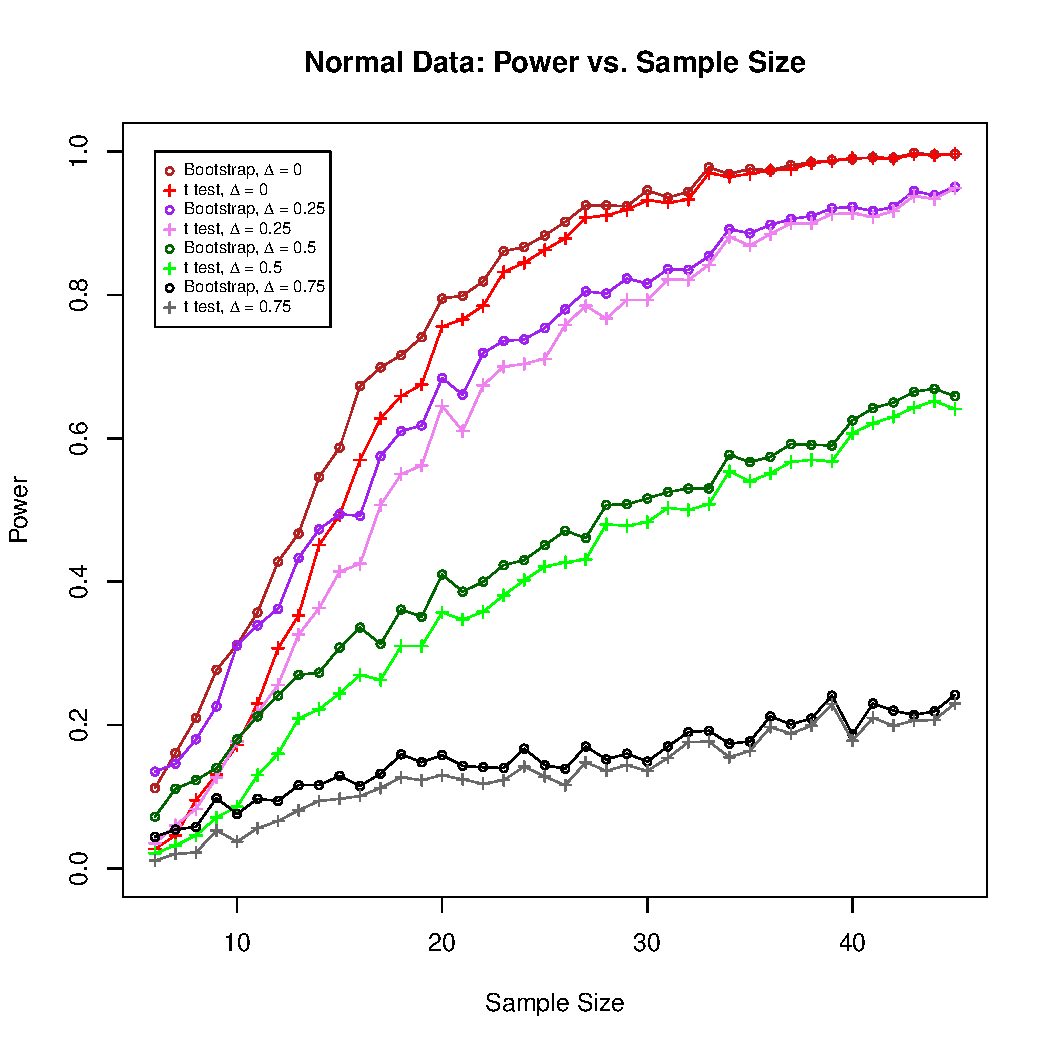
\includegraphics{NormalPowerEpsilon.pdf}
\caption{Normal data was divided into two groups, one with mean $0$ and the other with mean $\Delta$ as shown in the legend. Both groups have variance one. The bootstrap is represented with circles, and the t-test with crosses. Both tests reject the null if the 97.5\% confidence interval about the difference of means is not contained in $(-1,1)$}
\label{NormalPowerEpsilon}
\end{figure}

\pagebreak

\begin{figure}[h!]

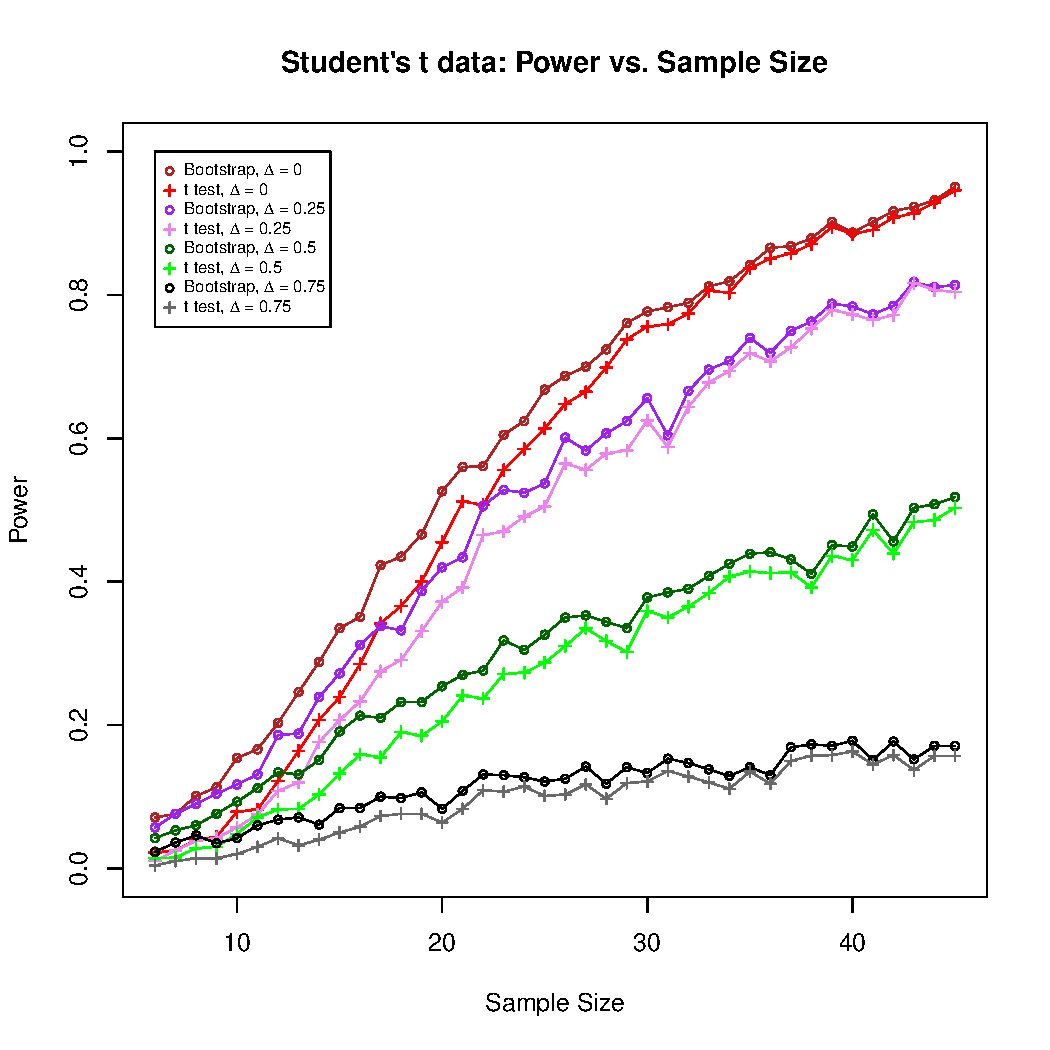
\includegraphics{Student'sTPowerEpsilon.pdf}

\caption{Student's $t$ data with six degrees of freedom was divided into two groups, one linearly shifted $\Delta$ away from zero, as shown in the legend. The bootstrap is represented with circles, and the t-test with crosses. Both tests reject the null if the 97.5\% confidence interval about the difference of means is not contained in $(-1, 1)$}
\end{figure}

\pagebreak

Against expectations, the bootstrap out-performs the t-test for normal data until the two reach agreement with high sample sizes (see figure \ref{NormalPowerEpsilon}). The difference is most pronounced for very small sample sizes and values of $D$ firmly inside the interval $( -\epsilon, \epsilon)$. As $D$ grows closer to $\epsilon$, the power of both tests decreases. The difference in powers also decreases as $D$ approaches $\epsilon$, as evidenced by their near-equally dismal power at $D = 0.75$. For normal data the average difference in power | that is the sample average of $\Pi_B - \Pi_{\mbox{\tiny{t-test}}}$ over sample sizes between six and twenty and twenty and forty five is given by:

\begin{eqnarray}
\label{table: normaldataPowerdifference}
\begin{tabular}{r | r  r r}
             & D = 0 & D = 0.25 & D = 0.5 \\ \hline
n $\leq$ 20  & 0.0813 & 0.077 & 0.0575  \\
n $> 20$ & 0.0061 & 0.0136 & 0.02475   \\
\end{tabular}
\end{eqnarray}


If the computing power is available and the data is normal there is evidently a clear advantage to using the bootstrap over the t-test, especially in circumstances with small data sets.

%\pagebreak

When applied to Student's $t$ distributed data, the performance of both tests decreased. The bootstrap continued to have greater power than the t-test, but by a smaller margin. For Student's $t$ data, the sample average of $\Pi_B - \Pi_{\mbox{\tiny{t-test}}}$ over sample sizes between six and twenty and then twenty and forty five is given by:

\begin{eqnarray}
\label{table: studentstdataPowerdifference}
\begin{tabular}{r | r  r r}
             & D = 0 & D = 0.25 & D = 0.5 \\ \hline
n $\leq$ 20  & 0.0663 & 0.05475 & 0.0435  \\
n $> 20$ & 0.0144 &0.01775 & 0.023   \\
\end{tabular}
\end{eqnarray}

Once again, there is a clear advantage to using the bootstrap over the t-test, but it is  slightly less pronounced as with normal data.

These results are unexpected to say the least. We would expect the satisfaction of the normal assumptions upon which the t-test relies to grant it advantage over the bootstrap. That it does not is cause for concern, and possibly an indication of an error in methodology. However, at the time of this writing, none could be found.







